
    \documentclass{standalone}
\usepackage{tkz-fct}
\usepackage{tkz-euclide}
\usepackage{color}
\renewcommand*\familydefault{\sfdefault}
\usepackage{sansmath}
\sansmath
\definecolor{gray75}{gray}{0.75}
\begin{document}
 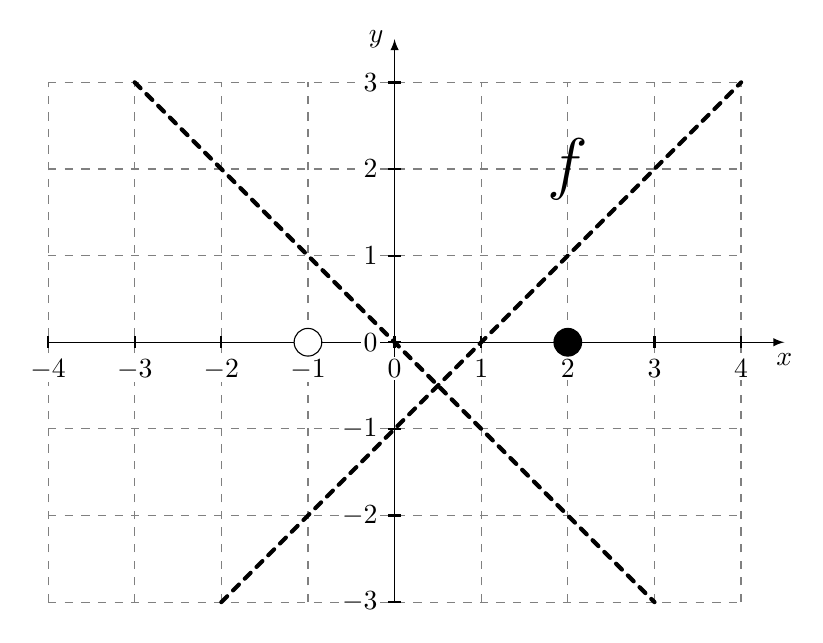
\begin{tikzpicture}[scale=1.1]
   \tkzInit[xmax=4.0,ymax=3.0,xmin=-4.0 ,ymin=-3.0]
   \begin{scope}[dashed]
     \tkzGrid
   \end{scope}
   \tkzDrawX[label={$x$}]
   \tkzDrawY[label={$y$}]
   \tkzLabelX
   \tkzLabelY
   \tkzFctPar[line width=2pt,samples=400,domain=0:1]{((1981583836043019*t**3 - 7475975381435025*t**2 + 10448351135499552*t - 7205759403792794)/2251799813685248)}{(-3*(t - 1)*(3602879701896397*t**2 - 4923935592591744*t + 9007199254740992)/9007199254740992)}
\tkzFctPar[line width=2pt,samples=400,domain=0:1]{((1801439850948199*t**3 + 1261007895663738*t**2 + 1441151880758559*t + 4503599627370496)/2251799813685248)}{(t*(10088063165309911*t**2 - 7926335344172070*t + 23058430092136935)/9007199254740992)}


                \tkzDefPoint(-3.0,3.0){A}

                \tkzDefPoint(3.0,-3.0){B}

                \tkzDrawSegment[style=dashed,line width = 1.5pt](A,B)


                \tkzDefPoint(-2.0,-3.0){A}

                \tkzDefPoint(4.0,3.0){B}

                \tkzDrawSegment[style=dashed,line width = 1.5pt](A,B)


   \tkzDrawPoint[size=10,color=black,fill=black](2.0,0.0)
\tkzDrawPoint[size=10,color=black,fill=white](-1.0,0.0)


   \tkzText(2,2){\Huge$f$}

\end{tikzpicture}
\end{document}
